\documentclass[20pt,usenames,dvipsnames]{beamer}\usepackage[]{graphicx}\usepackage[]{color}
% maxwidth is the original width if it is less than linewidth
% otherwise use linewidth (to make sure the graphics do not exceed the margin)
\makeatletter
\def\maxwidth{ %
  \ifdim\Gin@nat@width>\linewidth
    \linewidth
  \else
    \Gin@nat@width
  \fi
}
\makeatother

\definecolor{fgcolor}{rgb}{0.345, 0.345, 0.345}
\newcommand{\hlnum}[1]{\textcolor[rgb]{0.686,0.059,0.569}{#1}}%
\newcommand{\hlstr}[1]{\textcolor[rgb]{0.192,0.494,0.8}{#1}}%
\newcommand{\hlcom}[1]{\textcolor[rgb]{0.678,0.584,0.686}{\textit{#1}}}%
\newcommand{\hlopt}[1]{\textcolor[rgb]{0,0,0}{#1}}%
\newcommand{\hlstd}[1]{\textcolor[rgb]{0.345,0.345,0.345}{#1}}%
\newcommand{\hlkwa}[1]{\textcolor[rgb]{0.161,0.373,0.58}{\textbf{#1}}}%
\newcommand{\hlkwb}[1]{\textcolor[rgb]{0.69,0.353,0.396}{#1}}%
\newcommand{\hlkwc}[1]{\textcolor[rgb]{0.333,0.667,0.333}{#1}}%
\newcommand{\hlkwd}[1]{\textcolor[rgb]{0.737,0.353,0.396}{\textbf{#1}}}%
\let\hlipl\hlkwb

\usepackage{framed}
\makeatletter
\newenvironment{kframe}{%
 \def\at@end@of@kframe{}%
 \ifinner\ifhmode%
  \def\at@end@of@kframe{\end{minipage}}%
  \begin{minipage}{\columnwidth}%
 \fi\fi%
 \def\FrameCommand##1{\hskip\@totalleftmargin \hskip-\fboxsep
 \colorbox{shadecolor}{##1}\hskip-\fboxsep
     % There is no \\@totalrightmargin, so:
     \hskip-\linewidth \hskip-\@totalleftmargin \hskip\columnwidth}%
 \MakeFramed {\advance\hsize-\width
   \@totalleftmargin\z@ \linewidth\hsize
   \@setminipage}}%
 {\par\unskip\endMakeFramed%
 \at@end@of@kframe}
\makeatother

\definecolor{shadecolor}{rgb}{.97, .97, .97}
\definecolor{messagecolor}{rgb}{0, 0, 0}
\definecolor{warningcolor}{rgb}{1, 0, 1}
\definecolor{errorcolor}{rgb}{1, 0, 0}
\newenvironment{knitrout}{}{} % an empty environment to be redefined in TeX

\usepackage{alltt}
\usepackage[size=a0, orientation=portrait, scale=1.2]{beamerposter} % scale multiplies the font size of document class i.e. 20 x 1.4 = 28
\usepackage{float,graphicx}
\usepackage{ragged2e}   %new code
\usepackage{siunitx}
\graphicspath{{images/}}
\usepackage{xcolor}
\usepackage{tcolorbox}
\tcbuselibrary{skins}
\usetheme{Frankfurt}
\usepackage{subcaption}
\usepackage{longtable}
% \usepackage[natbib=true,backend=bibtex,sorting=none,hyperref=true,style=nature,isbn=false,doi=true,eprint=false,url=false]{biblatex}
\usepackage[natbib=true,backend=bibtex,sorting=anyt,hyperref=true,style=nature,isbn=false,eprint=false,url=false]{biblatex}
\addbibresource{bib/exported_items.bib}
\renewcommand*{\bibfont}{\footnotesize}

% set tcolorbox options
\tcbset{                                               % custom tcolorbox  
        skin=enhanced,                                 
        frame style={fill=blue},                       % sets the frame color
        bottom=10pt,                                    % distance between the body text and the bottom frame
        top=10pt,                                      % distance between the body text and the top frame
        left=10pt,
        right=10pt,
        boxrule=0pt,                                   % frame width
        bottomtitle=10pt,                               % distance between the title text and the bottom title frame               
        toptitle=10pt,                                  % distance between the title text and the top title frame
        lefttitle=10pt,                                  % title text left margin
        righttitle=10pt
}  

% this gives new block environment with custom margins
\newenvironment<>{myblock}[1]{%
 \begin{actionenv}#2%
 \def\insertblocktitle{\leftskip=0pt\rightskip=0pt\vspace{5pt} #1\vspace{5pt}}%
 \par%
 \usebeamertemplate{block begin}\leftskip=10pt\rightskip=0pt\vspace{5pt}}
 {\par\vspace{10pt}\usebeamertemplate{block end}
 \end{actionenv}}

% custom block template
\setbeamertemplate{block begin}{%
 \vskip.75ex%
 \begin{beamercolorbox}[leftskip=18pt,rounded=true,colsep*=.75ex]{block title}%
  \usebeamerfont{block title}\insertblocktitle%
  \end{beamercolorbox}%
  \vskip.5ex %
  \usebeamerfont{block body}%
  \begin{beamercolorbox}[leftskip=18pt,wd=\linewidth,colsep*=.75ex,sep=.75ex,vmode]{block body}%
}
\setbeamertemplate{block end}{%
  \end{beamercolorbox}%
}

% % justify text and specify margins
\addtobeamertemplate{block begin}{}{\justifying \leftskip=12pt\rightskip=10pt\vspace{10pt}}  %new code

% % to reduce the spacing between blocks
\addtobeamertemplate{block begin}{\vskip +\bigskipamount}{}
\addtobeamertemplate{block end}{}{\vskip +\bigskipamount}

% yet another box with tikz
\newsavebox\blockbox
\newenvironment{mytikzbox}{%
  \begin{lrbox}{\blockbox}%
    \begin{minipage}{0.99\textwidth} % this is because ".1" is sacrificed later in columns also
}{
    \end{minipage}
  \end{lrbox}
  \tikz\node[
    fill=green!60!blue!10,
    draw=black!50,
    line width=8pt,
    inner sep=7.5pt,
    rounded corners,
    outer sep=2pt,
    left=4pt,
    right=4pt
  ]{\usebox\blockbox};
}

% define some colors and set theme colors
\definecolor{afu-logo-color}{RGB}{48,220,43}
\definecolor{darkblue}{RGB}{0,0,255}
\setbeamercolor{background canvas}{bg=green!75}
\setbeamercolor{colorheadlinemine}{fg=white, bg=olive}

% create headline
\setbeamertemplate{headline}{%
\color{darkblue}\rule{\paperwidth}{20pt}
\begin{beamercolorbox}[wd=\paperwidth,rounded=true,shadow=true,leftskip=1.0cm,rightskip=1.0cm,colsep*=.75ex]{colorheadlinemine}
\begin{columns}

  \begin{column}{0.15\linewidth}
      \centering
      {\fontsize{40}{52}\selectfont Agriculture and Forestry University} \\
      
\includegraphics[width=0.85\linewidth]{afu-logo}
  \end{column}

  \begin{column}{0.85\linewidth} 
  \vskip10mm
  \centering\bfseries
  {\fontsize{80}{96}\selectfont Post anthesis leaf health as potential determinant of yield in early evaluation trial of wheat genotypes} \\[6mm]
  {\fontsize{60}{72}\selectfont Deependra Dhakal} \\[6mm]
  {\fontsize{48}{60}\selectfont Department of Plant Breeding, Agriculture and Forestry University} \\[3mm]
  {\fontsize{36}{42}\selectfont Bharatpur, Chitwan} \\[3mm]
  {\fontsize{36}{42}\selectfont Email: \url{ddhakal.rookie@gmail.com}} \\[3mm]
  \end{column}

\end{columns}
\end{beamercolorbox}

\color{darkblue}\rule{\paperwidth}{20pt}
}

% set footline
\setbeamercolor{colorfootlinemine}{fg=white, bg=red!20}
\setbeamertemplate{footline}{
\begin{beamercolorbox}[wd=\paperwidth,ht=1cm]{colorfootlinemine}
\centering
  {\small For highlights of my work: \url{ddhakal.rookie@gmail.com}}
\end{beamercolorbox}
}
\IfFileExists{upquote.sty}{\usepackage{upquote}}{}
\begin{document}
\begin{frame}[t]

\begin{mytikzbox}

{\bfseries Abstract} \\
Recent advances in phenotyping and statistical techniques have enabled exploration of a large number of trait in a greater depth. Current study undertaken in Agriculture and Forestry University, Rampur, Chitwan highlights uses augmented row-column design for a small number of checks for estimation of genotypes' effect under a mixed modeling framework to uncovering association of wheat crops yield with the traits characterizing its leaf health (resistance to foliar disease, flag leaf greenness, leaf area under greenness (LAUG) and flag leaf relative chlorophyll content. Even though significant genotypes' effects were found for most traits, few yield component traits along with a number of crop architecture traits -- thousand kernel weight, plant height, flag leaf area, canopy temperature depression, days to heading and days to anthesis -- had significant variation due to blocking or environmental factors. Major leaf health traits that influenced yield were the leaf greenness and relative chlorophyll content. BLUP estimation and adjustment for fixed effects dictate that 68.9\% of the genotypic variation of entry genotypes in yield was explained by the full model (one having both blocking and leaf health components). This reveals that augmenting leaf health traits with structured blocking factors leads to improved yield estimates. Apart from the check variety Aditya, which gave the lowest yield ( $3.02 \pm 0.61$ \si{\tonne\per\hectare}), all other check varieties were similar (3.54 \si{\tonne\per\hectare}, 3.33 \si{\tonne\per\hectare}, 3.42 \si{\tonne\per\hectare}). However, they had more contrasting differences in Number of tillers \si{\per\meter^{2}}. Findings based on block adjusted random effect estimates suggest for inclusion of some entry genotypes, those having leaf traits characterizing good health and with high yielding characters, in advanced evaluation trials. Top ranking high yielding entry genotypes were: TRCH/SRTU//KACHU/3/KINGBIRD\#1, WHEAR/SOKOLL/4/PASTOR// MILAN/KAUZ/3/B $\ldots$ and MUNAL \#1*2/4/HUW234+ LR34/PRINIA//PBW3 $\ldots$
\end{mytikzbox}

\vspace{-2.5cm}

\begin{columns}[t]

%==============================col-1==================
\begin{column}{0.32\linewidth}

\begin{myblock}{Introduction}
% Several candidate characters have been proposed as putative traits for yield improvement, but only a few of them can actually be reliably used in planned improvement programs. 
Post-anthesis foliar health could be a proxy for determining final grain yield. It has a direct implication on grain filling behavior of a plant. Ideally, the contribution of pre-anthesis photosynthetic reserves to the final grain yield has been found to stall around 5\% to 10\% \cite{sharma1992duration}. A major fraction of total yield, therefore, is dependent upon the photosynthesis that occurs post-anthesis. Terminal leaves, particularly the flag leaf and the one directly below it, have significant contribution to genotypic variation in yield \cite{aslam1978photosynthesis} with respect to provisioning of assimilate to functionally active parts of plants including the storage organ(grain). Similarly, it is well known that various biotic agents, primarily diseases, sustain reduction in yield with pathways that relate to the effective photosynthetic surface area \cite{lopes2012stay}.
\end{myblock}

\begin{block}{Materials and methods}
Test material consisted of 104 diverse lines representing advanced genotypes screened for resistance to various diseases. Four check varieties – Aditya, Bhrikuti, Gautam and Tilottama -- released by NARC and adapted to a wide range of environmental conditions of Nepal were included alongside. Observations were kept for final yield and associated as well as morpho-phenological traits, that were potentially prolonging the leaf health during post-anthesis period.

Field was sown in Nov 24, 2016. Seeds were continuously sown within a row while maintaining standard 25 cm row-row distance. Field was divided into rectangular grid to assign genotypes into rows, columns, rowgroups and columngroup. The net plot area hosting 240 plots was 240 \si{meter^2} The irrigation was scheduled to best avoid pre-antheis moisture stress, as this has been implied in largest losses resulting in number of fertile florets and the final grain weight \cite{innes1981effect}. Standard interculture operations were followed with none pesticidal sprays.

Individual plots were sampled for making observations. At least four plant hills, except for visual scoring and making observations on plant-environment interacting response (eg. canopy temperature depression, soil temperature and soil moisture traits) where distinct protocol exists, were randomly selected and a few representative tiller from each hill were duely analysed.

A mixed linear model was fitted for each of the response variables $y$ using lme4 package \cite{bates2014fitting}. All model terms except for the check variety effects, which was considered as fixed because they are purposely selected, were expressed with random intercept terms for obtaining model parameters \cite{wolfinger1997recovering}. REML estimate of the parameters were obtained by a single call for both fixed and random effects terms. A general matrix structure representation in a linear mixed model with conditional distribution of $y$ given $\mathcal{B} =\beta$ can be represented as shown in Equation \eqref{eq:linear-mixed-form},

\begin{equation}
(y|\mathcal{B}) \approx \mathcal{N}(X\beta + Zb, \sigma^{2}W^{-1})
\label{eq:linear-mixed-form}
\end{equation}

where $Z$ is the $n \times q$ model matrix for the $q$-dimensional vector-valued random effects variable, $\mathcal{B}$, whose value we are fixing at $b$. The unconditional distribution of $\mathcal{B}$ is also multivariate normal with mean zero and a parameterized $q \times q$ variance-covariance matrix \cite{bates2014fitting}. For multiple comparison of fixed effects means and stepwise variable selection procedure, least squares means and confidence intervals were calculated by Satterthwaite approximation of degrees of freedom \cite{alexandra2017}.
\end{block}

\end{column}
%==============================col-2==================
\begin{column}{0.32\linewidth}

% \begin{tcolorbox}[title=test]
\begin{tcolorbox}[]
\begin{figure}[t!]
    \centering
    \begin{subfigure}[tb]{0.5\textwidth}
        \centering
        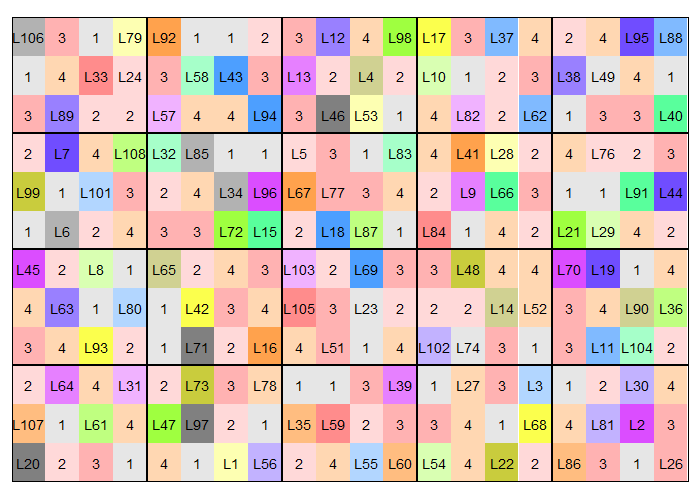
\includegraphics[height=3in]{design_layout}
        \caption{Randomized layout of the row-column experimental design}
    \end{subfigure}%
    ~ 
    \begin{subfigure}[tb]{0.5\textwidth}
        \centering
        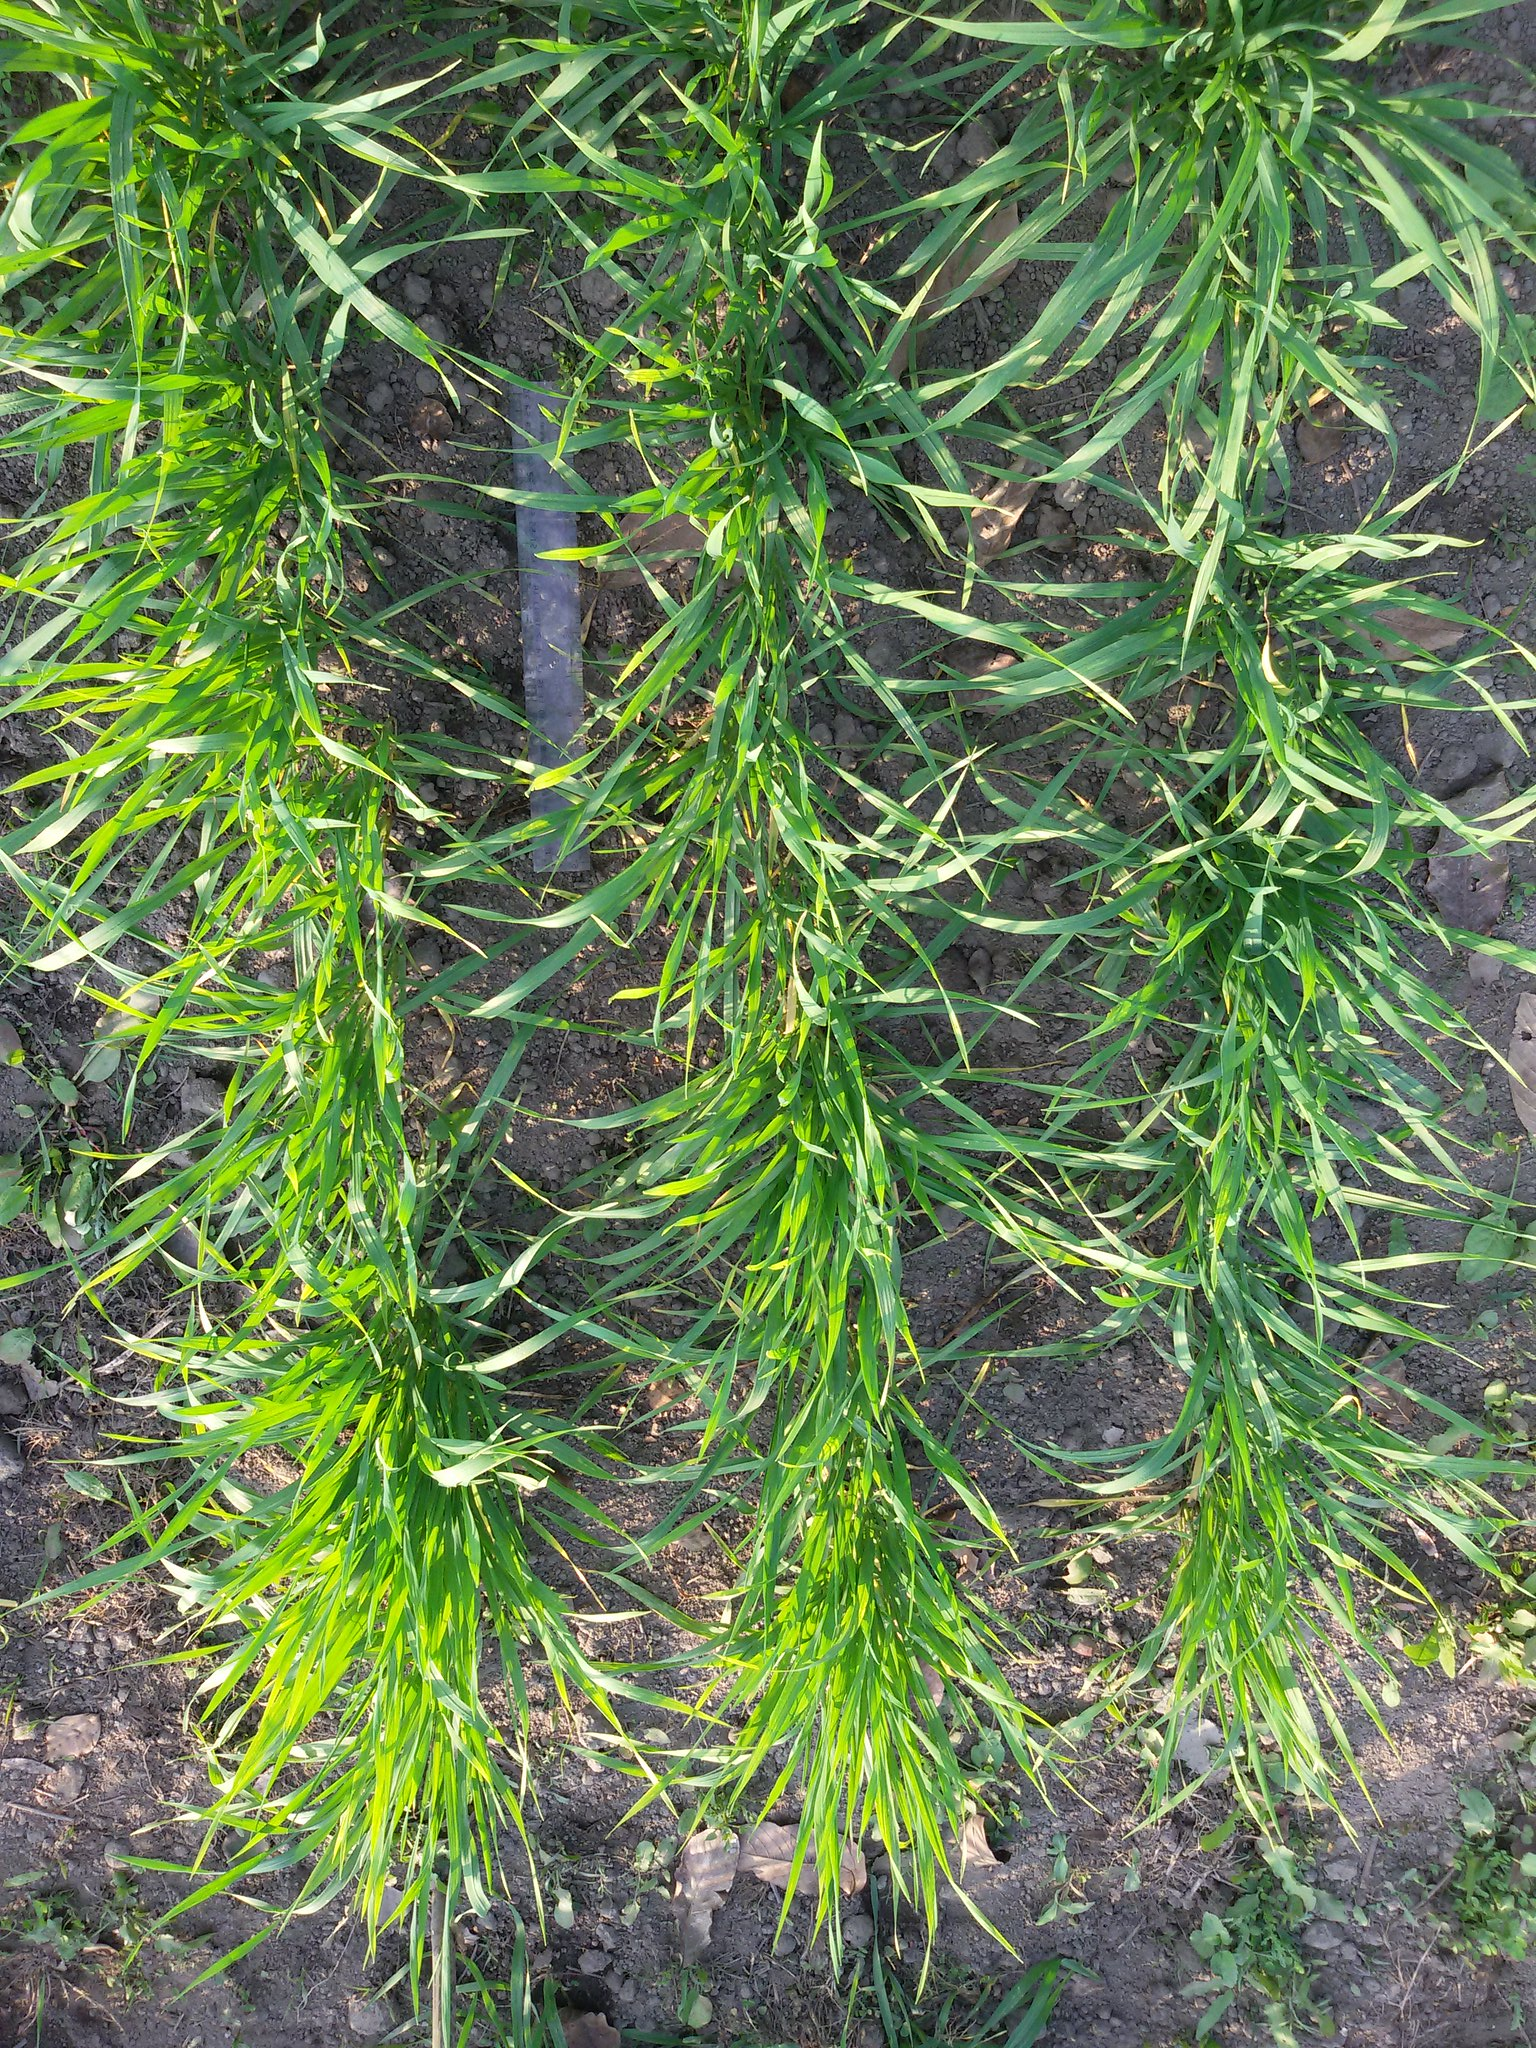
\includegraphics[height=4in]{34046350313_ff4f0341d0_k}
        \caption{Wheat crop plot at Jan 9, 2017 (46 days after sowing)}
    \end{subfigure}
    \caption{\centering Study design and crop canopy shown during recording of observation}
\end{figure}
\end{tcolorbox}

\begin{block}{Results}

Mixed model summary of fixed effects terms of yield and yield component traits

\begingroup
\tiny
\begin{longtable}{@{\extracolsep{1pt}}lccccc}
\\[-1.8ex]\hline
\hline \\[-1.8ex]
 & \multicolumn{5}{c}{\textit{Dependent variable:}} \\
\cline{2-6}
\\[-1.8ex] & \multicolumn{5}{c}{\textit{linear}} \\
 & \multicolumn{5}{c}{\textit{mixed-effects}} \\
 & Yield & \parbox[t]{2.5cm}{Number of effective tillers} & \parbox[t]{2.5cm}{Thousand kernel weight} & \parbox[t]{2.5cm}{Grains per panicle} & Panicle length \\
\\[-1.8ex] & (1) & (2) & (3) & (4) & (5)\\
\hline \\[-1.8ex]
 Bhrikuti & 0.52$^{***}$ (0.14) & 3.34$^{**}$ (1.35) & 1.17 (0.85) & $-$0.22 (0.49) & 0.51 (0.33) \\
  & p = 0.0003 & p = 0.02 & p = 0.17 & p = 0.66 & p = 0.13 \\
  Gautam & 0.31$^{**}$ (0.14) & 0.33 (1.36) & 2.06$^{**}$ (0.85) & 1.33$^{***}$ (0.49) & 1.22$^{***}$ (0.33) \\
  & p = 0.03 & p = 0.81 & p = 0.02 & p = 0.01 & p = 0.0003 \\
  Tilottama & 0.40$^{***}$ (0.14) & 6.94$^{***}$ (1.36) & $-$0.32 (0.85) & 0.38 (0.49) & 0.27 (0.33) \\
  & p = 0.005 & p = 0.0000 & p = 0.72 & p = 0.45 & p = 0.43 \\
  Aditaya (Constant) & 3.02$^{***}$ (0.61) & 26.80$^{***}$ (2.45) & 36.40$^{***}$ (4.32) & 27.00$^{***}$ (1.88) & 16.30$^{***}$ (1.09) \\
  & p = 0.0000 & p = 0.00 & p = 0.00 & p = 0.00 & p = 0.00 \\
 \hline \\[-1.8ex]
Observations & 202 & 238 & 201 & 202 & 226 \\
Log Likelihood & $-$209.00 & $-$752.00 & $-$575.00 & $-$452.00 & $-$414.00 \\
Akaike Inf. Crit. & 443.00 & 1,528.00 & 1,174.00 & 928.00 & 853.00 \\
Bayesian Inf. Crit. & 482.00 & 1,570.00 & 1,213.00 & 968.00 & 894.00 \\
\hline
\hline \\[-1.8ex]
\textit{Note:}  & \multicolumn{5}{r}{$^{*}$p$<$0.1; $^{**}$p$<$0.05; $^{***}$p$<$0.01} \\
\end{longtable}
\endgroup

The model with both genotypes (checks and entries) outperforms in comparison to the one without in predicting the real yield (\(\chi^2 = 14.4\) with \(df = 4\)).

Pairwise comparison of fixed effects estimate indicate that check variety Aditya has the lowest yield amongst all varieties while other have similar yields. Average yield of the lowest yielder is \(4.53\ tons\ ha^{-1}\ (\pm\ 0.60)\) and Bhrikuti yields the highest with average yield of \(5.04\ tons\ ha^{-1}\ (\pm\ 0.60)\). 

Genotypes show highly significant differences for the disease resistance trait. LRT shows that both checks and entries possess significant (\(\chi^2\) statistic=\(13.85\) with \(4\ df\)) heritable variation. Check variety Gautam is relatively asymptomatic (\(2.51\ (\pm\ 1.30)\)) than Bhrikuti(\(3.32\ (\pm\ 1.30)\)) and Tilottama (\(3.35\ (\pm\ 1.30)\)) varieties to foliar pathogen. Although, no distinction could be made on the severity scale of the disease (All check varieties exhibited similarly less affected (2.5-5.0) symptom at the time of scoring). Entry genotypes also show considerable amount of heritable variation.

Genotypes showed highly significant differences in the greenness score measured measured at Zadok's stages 75 and 85. LRT shows that both checks and entries possess significant heritable variation. Pairwise comparison of fixed effect estimates for both growth stages implicate check variety Aditya for retaining maximum greenness of the flag leaf followed by Bhrikuti and Gautam (both have similar greenness scores) and Tilottama. Noteworthy variation was also found among the entry genotypes (significant at \(p < 0.01\)). Check variety Aditya suffered largest reduction in greenness (\(93.03\ (\pm\ 19.70)\)), while Tilottama had the least (\(77.35\ (\pm\ 19.71)\)) loss of all check varieties. 

Highly significant difference exist among the genotypes for Plant height trait. However, the random effects estimates of plant height showed no difference among entry genotypes. No significant difference was discovered among the genotypes for flag leaf surface area trait, either. In contrast, entry genotypes' chlorophyll content at Zadok's stage 65 showed considerable variation, while the it is not true for check genotypes. 
\end{block}

\end{column}
%==============================col-3==================
\begin{column}{0.32\linewidth}

\begin{tcolorbox}[]

Significant differences were detected among the check genotypes but not among entries for the SPAD measured at Zadok's stage 85. Likewise, genotypes have significant differences for the Canopy temperature depression (CTD) measured near anthesis stage. Fixed effect estimates shows that canopy structure of check variety Bhrikuti favors greater reduction in temperature than check variety Aditya (\(9.08^\circ C\ (\pm\ 0.79)\)). Other varieties were at par with both of the check varieties. Highly significant difference were detected among the genotypes were found for days to heading trait. All check varieties differ from one another except for Aditya (late heading type) (with mean of \(67.79\ (\pm\ 2.40)\) days) and Gautam, which require similar days for heading. Mean number of days taken for head to develop in half of the population was lowest in Tilottama (\(62.71\ (\pm\ 2.40)\) days) variety. Similarly, entry genotype levels also exhibited high variation for the trait.

\begin{figure}[H]
\footnotesize
{\centering 
\subfloat[Yield\label{fig:yield-blup-viz-1}]{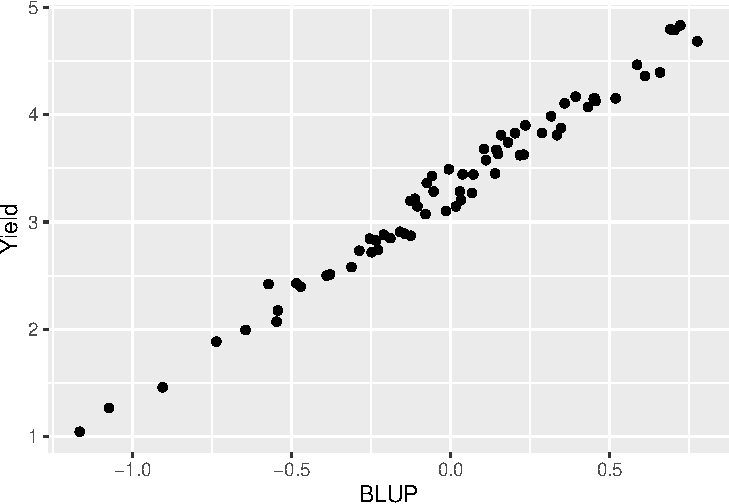
\includegraphics[width=.32\linewidth]{yield-blup-viz-1} }
\subfloat[Number of effective tillers\label{fig:yield-blup-viz-2}]{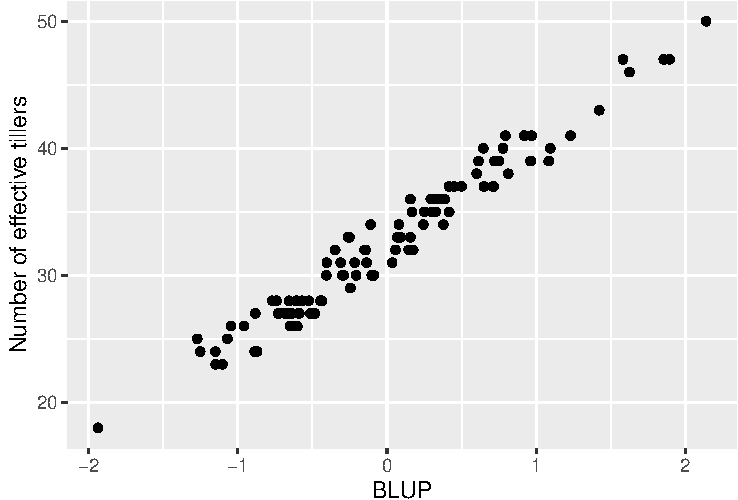
\includegraphics[width=.32\linewidth]{yield-blup-viz-2} }
\subfloat[Thousand kernel weight\label{fig:yield-blup-viz-3}]{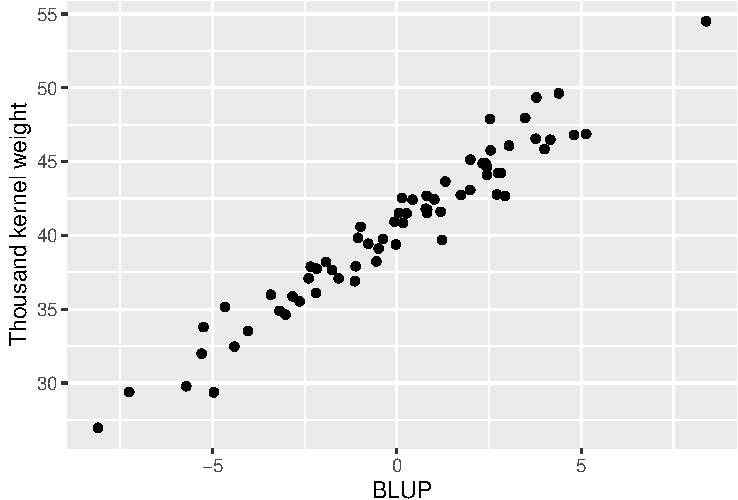
\includegraphics[width=.32\linewidth]{yield-blup-viz-3} }\newline
\subfloat[Number of grains per panicle\label{fig:yield-blup-viz-4}]{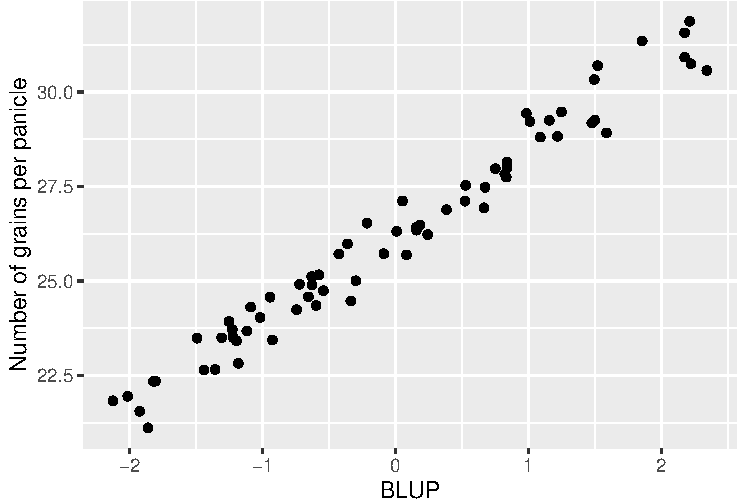
\includegraphics[width=.32\linewidth]{yield-blup-viz-4} }
\subfloat[Panicle length\label{fig:yield-blup-viz-5}]{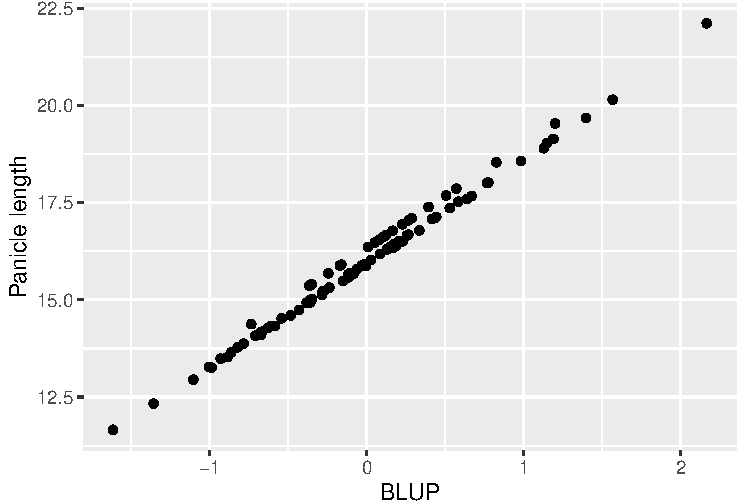
\includegraphics[width=.32\linewidth]{yield-blup-viz-5} }}
\caption{\centering Scatterplot of observed versus BLUP values of yield and yield component traits}\label{fig:yield-blup-viz}
\end{figure}

The coefficient of determination, between the observed and fitted values of random effects model are 0.61, 0.36, 0.71, 0.55, 0.48, respectively for the Yield, Number of effective tillers, Thousand kernel weight, Number of grains per panicle and Panicle length.

\begin{figure}[H]

{\centering 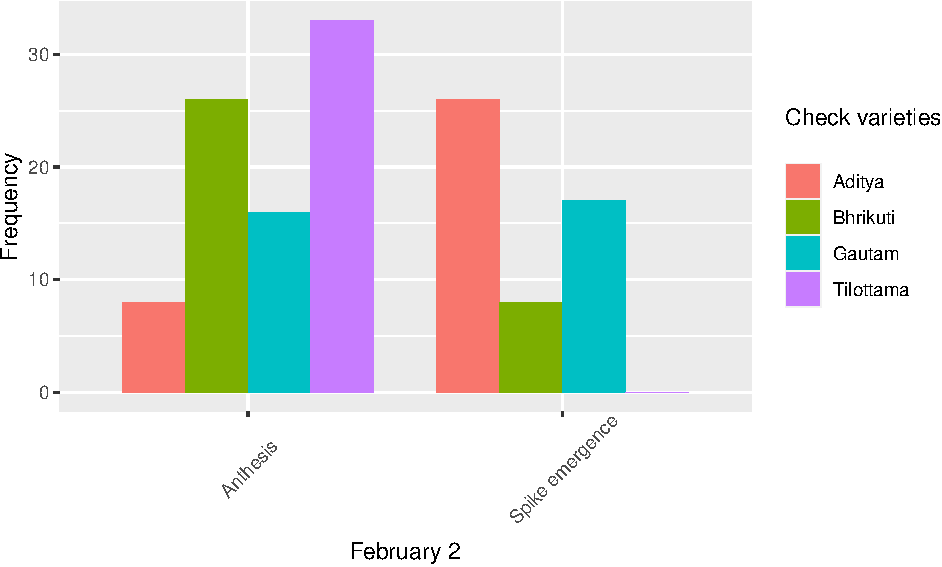
\includegraphics[width=0.60\linewidth]{cor-graph-barplot-viz-checks-1} 

}
\caption{Number of checks at different growth stages on February 2, 2017. Time point comparison of different stages of reproductive periods of growth reaffirms that Tilottama variety flowers the earliest amongst the check varieties and Aditya reaches to the flowering relatively late.}\label{fig:cor-graph-barplot-viz-checks}
\end{figure}
\end{tcolorbox}

\begin{block}{References}
\printbibliography
\end{block}


\end{column}
\end{columns}

\end{frame}
\end{document}
